%--------------------------------------------------------------------------
\chapter{}

%--------------------------------------------------------------------------
\section{Total Order in Webern's Op.~27}

\begin{example}
	\cite[207]{Starr1984}
	\label{starr-webern-example}
	This examples provides a strategy to unravel the basic total order in Webern's Op.~27. It is somewhat paradoxical in the sense that unveiling the row requires prior knowledge of it. Consider the opening bars in Webern's Op.~27 depicted in Fig.~\ref{fig:webern-27}, as well as their aggregate realization given in Fig.~\ref{fig:webern-aggregate}.

    \begin{figure}[htbp]
    	\centering
		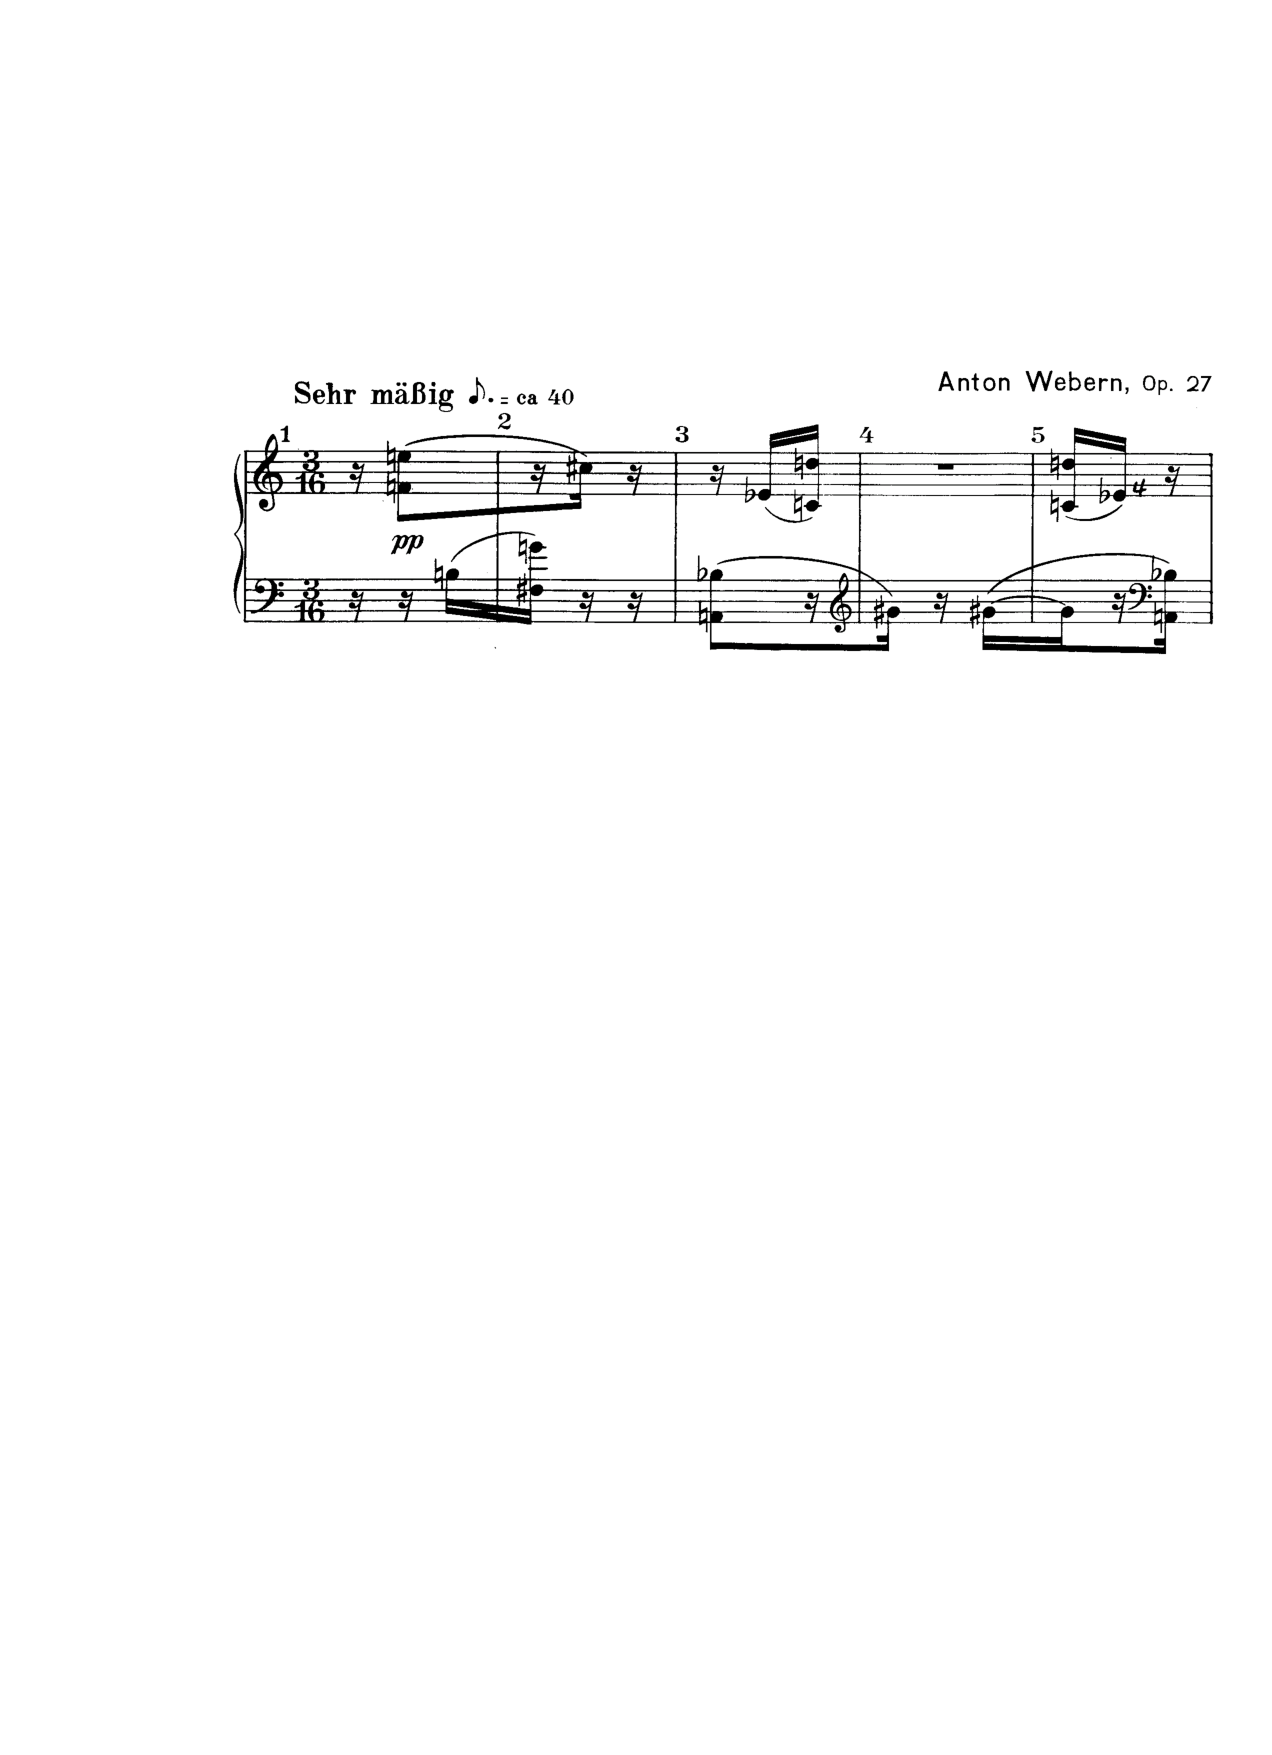
\includegraphics[width=6.5in]{figures/webern1.pdf}
		\caption[Bars 1--7 in Webern's Op.~27]{The initial bars in Webern's Op.~27.}
    	\label{fig:webern-27}
	\end{figure}

    \begin{figure}[htbp]
    	\centering
		\begin{tikzcd}
        	& E \arrow[dr] && G \arrow[dr] && B\flat \arrow[dr] && D \arrow[dr] & \\
        	* \arrow[dr] \arrow[ur] && B \arrow[dr] \arrow[ur] && C\sharp \arrow[dr] \arrow[ur] && E\flat \arrow[dr] \arrow[ur] && G\sharp \\
        	& F \arrow[ur] && F\sharp \arrow[ur] && A \arrow[ur] && C \arrow[ur] &
    	\end{tikzcd}
		\caption[Aggregate Realization of Bars 1--7 in Webern's Op.~27]{An aggregate realization of the initial bars in Webern's Op.~27. At its very first presentation, the total order used to generate the piece cannot be discerned. Moreover, the partial order that can actually be heard intercalates the total order's two hexachords, a procedure that can be construed as a form of derivation.}
    	\label{fig:webern-aggregate}
	\end{figure}

	\noindent Instead of the aggregate realization in Fig.~\ref{fig:webern-aggregate}, however, the fact that the basic series is known to be $S = \{ 4, 5, 1, 3, 0, 2, 8, 9, 10, 6, 7, 11 \}$ is used take the initial bars seen in Fig.~\ref{fig:webern-27}, and rewrite an aggregate realization, call it $D_1$, of them as in Fig.~\ref{fig:webern-aggregate-b}.

	\begin{figure}[htbp]
    	\centering
		\begin{tikzcd}
	    	& [-1em] E \arrow[dr] & [-1em] & [-1em] & [-1em] D \arrow[rd] & [-1em] & [-1em] B\flat \arrow[dr] & [-1em] & [-1em] G \arrow[dr] & [-1em] \\
	    	* \arrow[dr] \arrow[ur] & [-1em] & [-1em] C\sharp \arrow[r] & [-1em] E\flat \arrow[dr] \arrow[ur] & [-1em] & [-1em] G\sharp \arrow[dr] \arrow[ur] & [-1em] & [-1em] * \arrow[dr] \arrow[ur] & [-1em] & [-1em] B \\
	    	& [-1em] F \arrow[ur] & [-1em] & [-1em] & [-1em] C \arrow[ur] & [-1em] & [-1em] A \arrow[ur] & [-1em] & [-1em] F\sharp \arrow[ur] & [-1em]
    	\end{tikzcd}
    	\caption[Another Aggregate Realization of Bars 1--7 in Webern's Op.~27]{The underlying partial order depicted in this aggregate realization is denoted by $D_1$.}
    	\label{fig:webern-aggregate-b}
	\end{figure}

	\noindent It is not too far-fetched to assume such an analysis. Whereas Fig.~\ref{fig:webern-aggregate} represented a first-time hearing depiction of bars 1--7, Fig.~\ref{fig:webern-aggregate-b} can be achieved by, say, a performer who realizes the voice-crossing of the series along its reflection axis. Having come to this conclusion, parsing bars 8--10 becomes a bit less daunting. Fig.~\ref{fig:webern-27-b} shows bars 8--10 in Op.~27, and Fig.~\ref{fig:webern-aggregate-c} is a normalized aggregate realization of the passage. Normalized here means that the series being displayed in the music is $\T_{10}\I(S) = \{ 6, 5, 9, 7, 10, 8, 2, 1, 0, 4, 3, 11 \}$, but instead the aggregate realization is set to $S$, in order to facilitate taking intersections of both partial orders later. $\T_{10}\I(S)$ begins with the right hand in bar 8, moves to the left hand in bar 9, and the very last note (which is not showing) is a high B the right hand again has in bar 11. At this point, any confidence that a series can be heard by the listener is severely damaged. It is unlikely that the average performer will have obtained, or even cared to obtain, a good grasp on what the series really is.

	\begin{figure}[htbp]
    	\centering
		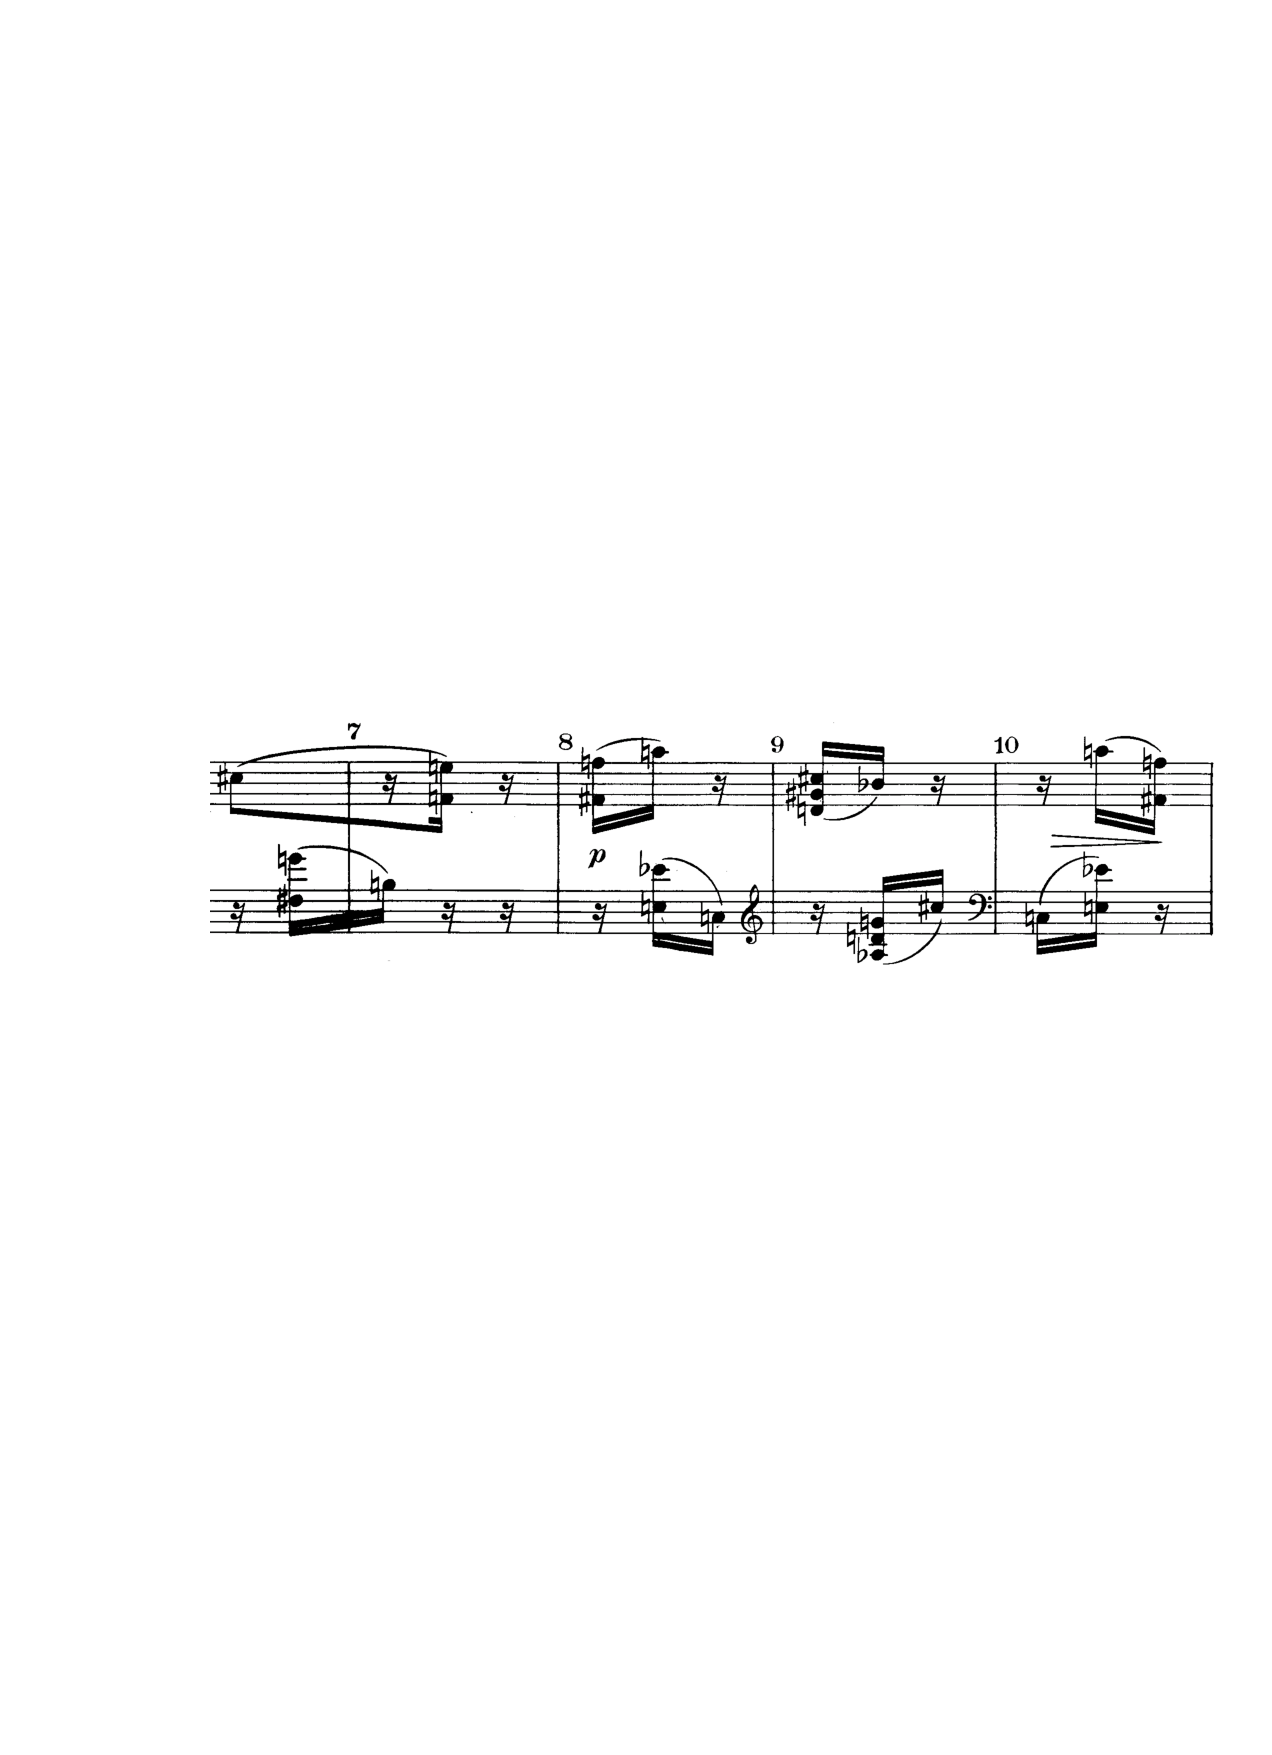
\includegraphics[width=6.5in]{figures/webern2.pdf}
		\caption[Bars 8--10 in Webern's Op.~27]{Bars 8--10 in Webern's Op.~27.}
    	\label{fig:webern-27-b}
	\end{figure}

	\begin{figure}[htbp]
    	\centering
		\begin{tikzcd}
	    	&&& E\flat \arrow[ddr] &&&& \\
	    	& E \arrow[dr] && D \arrow[dr] &&& G \arrow[dr] & \\
	    	* \arrow[ur] \arrow[dr] && C\sharp \arrow[ur] \arrow[dr] \arrow[uur] \arrow[ddr] && A \arrow[r] & B\flat \arrow[ur] \arrow[dr] && B \\
	    	& F \arrow[ur] && C \arrow[ur] &&& F\sharp \arrow[ur] & \\
	    	&&& G\sharp \arrow[uur] &&&&
    	\end{tikzcd}
		\caption[An Aggregate Realization of Bars 8--10 in Webern's Op.~27]{The underlying partial order depicted in this aggregate realization is denoted by $D_2$.}
    	\label{fig:webern-aggregate-c}
	\end{figure}

	\noindent The next excerpt analyzed in the first movement is the last one needed in order to infer what series Webern used for the piece. The musical passage, taken from bars 19--23, is given in Fig.~\ref{fig:webern-27-c}, and an aggregate realization is displayed in Fig.~\ref{fig:webern-aggregate-d}. It is again normalized with respect to $S$. This time, the series being sought in the excerpt is $\T_3\I(S) = \{ 11, 10, 2, 0, 3, 1, 7, 6, 5, 9, 8, 4 \}$, and again it has a very convoluted presentation, floating around in register, and freely changing hands. This fact emphasizes the realization that, without the score, it is unlikely that a listener, even a very educated one, will be able to discern the composer's main generative material by hearing alone.

	\begin{figure}[htbp]
    	\centering
		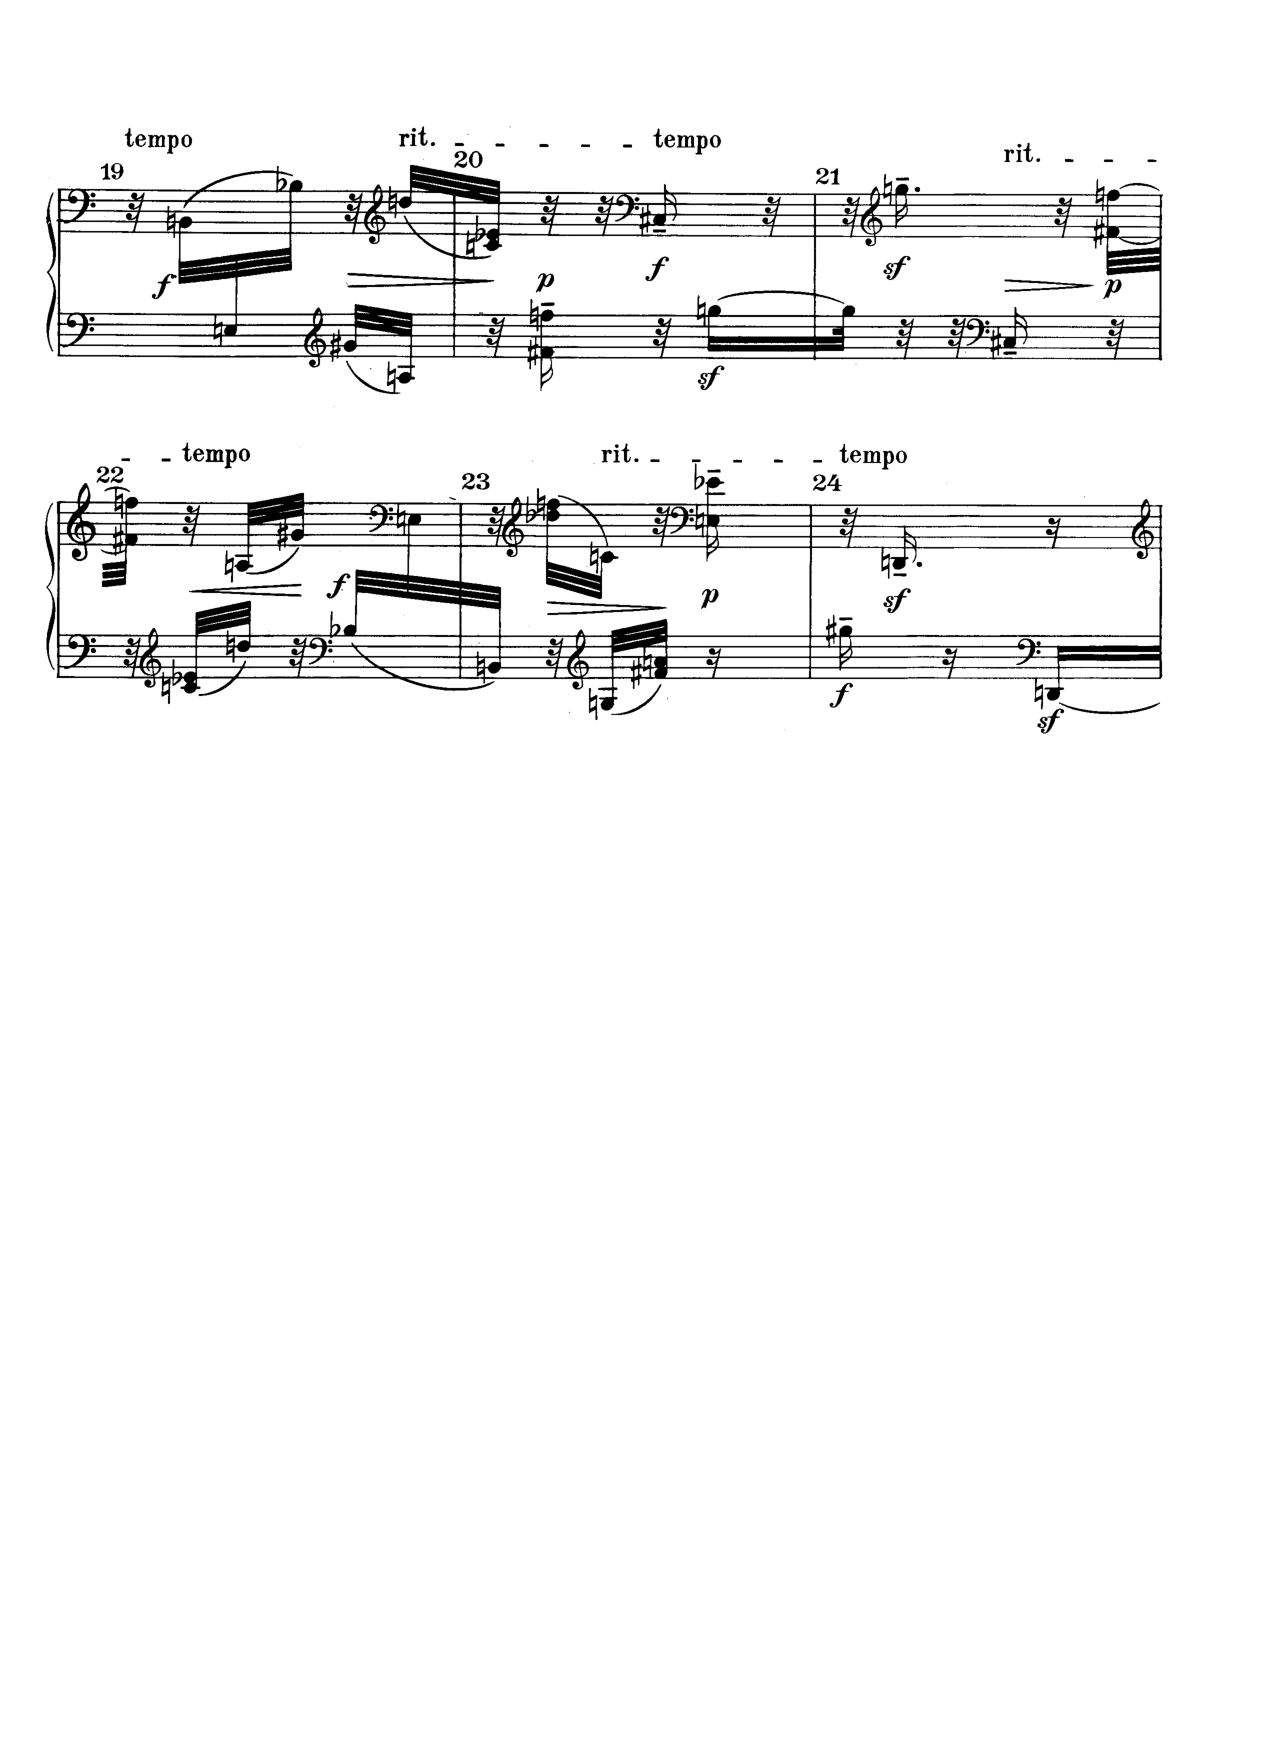
\includegraphics[width=6.5in]{figures/webern3.pdf}
		\caption[Bars 19--23 in Webern's Op.~27]{Bars 19--23 in Webern's Op.~27.}
    	\label{fig:webern-27-c}
	\end{figure}

	\begin{figure}[htbp]
    	\centering
		\begin{tikzcd}
	    	& [-1em] & [-1em] & [-1em] E\flat \arrow[dr] & [-1em] & [-1em] & [-1em] B\flat \arrow[dr] & [-1em] & [-1em] & [-1em] \\
	    	E \arrow[r] & [-1em] F \arrow[r] & [-1em] C\sharp \arrow[ur] \arrow[dr] & [-1em] & [-1em] D \arrow[r] & [-1em] G\sharp \arrow[ur] \arrow[dr] & [-1em] & [-1em] F\sharp \arrow[r] & [-1em] G \arrow[r] & [-1em] B \\
	    	& [-1em] & [-1em] & [-1em] C \arrow[ur] & [-1em] & [-1em] & [-1em] A \arrow[ur] & [-1em] & [-1em] & [-1em]
    	\end{tikzcd}
		\caption[An Aggregate Realization of Bars 19--23 in Webern's Op.~27]{The underlying partial order depicted in this aggregate realization is denoted by $D_3$.}
    	\label{fig:webern-aggregate-d}
	\end{figure}

	\noindent The last step in figuring out Webern's total order, according to the theoretical assumptions made so far, is to take intersections of the partial orders depicted above with aggregate realizations. Assuming the presentation of the series could actually be heard despite the numerous pitfalls represented by all the registral displacements in the piece, and furthermore assuming twelve ordered and different pitch classes could be freely inverted and transposed by ear almost instantly, the intersection $D_1 \cap D_2$ at measure 10 would possibly be inferred. An aggregate realization of the intersection is shown in Fig.~\ref{fig:webern-aggregate-e}. However, since there would still be three incomparabilities that preventing full comprehension the underlying series.

	\begin{figure}[htbp]
    	\centering
		\begin{tikzcd}
	    	& [-1em] E \arrow[dr] & [-1em] & [-1em] & [-1em] D \arrow[dr] & [-1em] & [-1em] & [-1em] & [-1em] G \arrow[dr] & [-1em] \\
	    	* \arrow[ur] \arrow[dr] & [-1em] & [-1em] C\sharp \arrow[r] & [-1em] E\flat \arrow[ur] \arrow[dr] & [-1em] & [-1em] G\sharp \arrow[r] & [-1em] A \arrow[r] & [-1em] B\flat \arrow[ur] \arrow[dr] & [-1em] & [-1em] B \\
	    	& [-1em] F \arrow[ur] & [-1em] & [-1em] & [-1em] C \arrow[ur] & [-1em] & [-1em] & [-1em] & [-1em] F\sharp \arrow[ur] & [-1em] \\
    	\end{tikzcd}
		\caption[Intersecting Bars 1--7 with Bars 8--10 in Webern's Op.~27]{The intersection $D_1 \cup D_2$.}
    	\label{fig:webern-aggregate-e}
	\end{figure}

	\noindent The next two pictures depict aggregate realizations for the intersections $D_1 \cap D_3$ and $D_2 \cap D_3$. Having reached measure 23, Webern's series can finally be obtained. Both intersections, however, still carry incomparabilities, so taking the intersection of all three aggregate realizations is still necessary.

	\begin{figure}[htbp]
    	\centering
		\begin{tikzcd}
	    	& [-1em] & [-1em] & [-1em] & [-1em] & [-1em] & [-1em] & [-1em] B\flat \arrow[dr] & [-1em] & [-1em] & [-1em] \\
	    	E \arrow[r] & [-1em] F \arrow[r] & [-1em] C\sharp \arrow[r] & [-1em] E\flat \arrow[r] & [-1em] C \arrow[r] & [-1em] D \arrow[r] & [-1em] G\sharp \arrow[ur] \arrow[dr] & [-1em] & [-1em] F\sharp \arrow[r] & [-1em] G \arrow[r] & [-1em] B \\
	    	& [-1em] & [-1em] & [-1em] & [-1em] & [-1em] & [-1em] & [-1em] A \arrow[ur] & [-1em] & [-1em] & [-1em]
    	\end{tikzcd}
		\caption[Intersecting Bars 1--7 with Bars 19--23 in Webern's Op.~27]{The intersection $D_1 \cup D_3$.}
    	\label{fig:webern-aggregate-f}
	\end{figure}

	\begin{figure}[htbp]
    	\centering
		\begin{tikzcd}
	    	& [-1em] & [-1em] & [-1em] E\flat \arrow[dr] & [-1em] & [-1em] & [-1em] & [-1em] & [-1em] & [-1em] & [-1em] \\
	    	E \arrow[r] & [-1em] F \arrow[r] & [-1em] C\sharp \arrow[ur] \arrow[dr] && [-1em] D \arrow[r] & [-1em] G\sharp \arrow[r] & [-1em] A \arrow[r] & [-1em] B\flat \arrow[r] & [-1em] F\sharp \arrow[r] & [-1em] G \arrow[r] & [-1em] B \\
	    	& [-1em] & [-1em] & [-1em] C \arrow[ur] & [-1em] & [-1em] & [-1em] & [-1em] & [-1em] & [-1em] & [-1em]
    	\end{tikzcd}
		\caption[Intersecting Bars 8--10 with Bars 19--23 in Webern's Op.~27]{The intersection $D_2 \cup D_3$.}
    	\label{fig:webern-aggregate-g}
	\end{figure}

	\begin{figure}[htbp]
    	\centering
		\begin{tikzcd}
	    	E \arrow[r] & [-1em] F \arrow[r] & [-1em] C\sharp \arrow[r] & [-1em] E\flat \arrow[r] & [-1em] C \arrow[r] & [-1em] D \arrow[r] & [-1em] G\sharp \arrow[r] & [-1em] A \arrow[r] & [-1em] B\flat \arrow[r] & [-1em] F\sharp \arrow[r] & [-1em] G \arrow[r] & [-1em] B
    	\end{tikzcd}
		\caption[The intersection of Bars 1--7, 8--10, and 19--23 in Webern's Op.~27]{The intersection $D_1 \cup D_2 \cup D_3$.}
    	\label{fig:webern-aggregate-h}
	\end{figure}
\end{example}

There is much to be said about Ex.~\ref{starr-webern-example}, particularly in what regards the aural perception of the composer's constructs. There is even more to be said when taking into consideration the fact that, as the twentieth-century unraveled, it became in many cases increasingly more difficult to establish how a piece of music was constructed with the presence of the score alone, much less simply by aural inference. It becomes less straightforward to determine the role of the listener in these cases, especially whenever one insists that the listener should be able to aurally infer \emph{every} construct in a musical composition. It can be argued that, as composers differentiate themselves from common practice, compositional technique becomes more subjective, and often indiscernible in the musical discourse. That does not mean, however, that musical fruition should be hindered in any sense, or that the composer's channel of communication with the listener has been narrowed in any way. It is simply the case that, even when not every single part of a structure is fathomed, the structure itself can still be experienced.

%We do not need a blueprint to live in a house, we do not need a wrench to drive a car, and we certainly do not begin to understand the intricacies of the very universe in which we exist. And we do exist nonetheless.

The role of the analyst, on the other hand, also becomes more difficult to define. Whenever the structure of a piece of music becomes impossible to follow from its score alone, a theorist must reconsider the weight of musicological work in the analysis of such repertoire. In other words, it may very well be impossible to analyze a composition without resorting to the composer, or to a musicological study thereof. That is especially the case with algorithmic composition, which is a major avenue to which we shall apply our main object of study. Analyzing an algorithmically generated piece of music without prior knowledge of the algorithm itself can only go as far as devising hearing strategies for the piece, as well as conjecturing what the algorithm might have been. It may be of substantial value, it may even carry more value than an analysis of the algorithm itself. And, just like with any piece of software, understanding the code is not a prerequisite to using said software, much less to determining whether it fulfills its purpose, or whether it is a good piece of software or not. However, if one intends to determine precisely how a piece of music was \emph{constructed}, then knowledge of its blueprint becomes essential. And that determination is often of primary interest to composers.

The compositional techniques we are about to define and generalize in this study are notoriously of structural relevance. It does not mean that they cannot be aurally discerned, and in fact many authors devote considerable time devising hearing strategies for them, particularly when they are used to structure pitch. Nevertheless, our approach here will be restricted to the intrinsic qualities of these techniques, and we shall not pursue their aural perception in depth, simply because there may not be any intention from the composer's part for them to be heard at all. A familiar example might be the music of Stravinsky. Upon analyzing his use of rotational arrays, it becomes clear that the composer uses them as a generative techniques, rather than as a foreground musical entities. Analyzing such pieces often resort to techniques that have no connection whatsoever to any sort of hearing strategy, like Forte's employment of K and Kh set complexes, which yield a nexus set that ultimately cannot be heard. We aggravate this discussion with the idea that, more often than not, we shall employ the techniques we are about to present to dimensions other than pitch, and in particular to algorithmically determining spectral components and timbre. In this sense, their outcomes become textural elements of a composition, but still well within the canon of tasks a composer needs to exercise in the craft of a piece.

That being said, neither the above techniques addresses self-derivation's primary concern: given a set of order numbers and a transformation, what series are capable of producing transforms of \emph{themselves} when pulled from those order numbers. This is in essence the exact opposite of what was demonstrated above, where we depart from a series and attempt to understand its embedded segments. And it is arguably not a coincidence, as much of the twelve-tone theory devised since Forte has a strong analytical bias. What we are mainly interested, however, is in how these techniques fit onto the compositional scheme of things. And for that, having a two-way street where, on one hand we understand raw compositional materials and, on the other, we formulate them, is crucial. Moreover, as we attempt to construe orderedness as a generative procedure in all generality, it becomes imperative that we break our ties with purely analytical music theory and begin to delve into the mathematics of these general constructs. As the example below suggests, mathematics can greatly simplify the way we approach certain concepts and, depending on the task at hand, may even be decisive in determining whether it is feasible or not to pursue certain compositional avenues. For algorithmic composition, in particular, having a firm theoretical understanding of some generative procedure can greatly simplify the composer's algorithm, as well as make it more efficient.
